\documentclass[../../../main.tex]{subfiles}
\begin{document}
As demonstrated in the previous section, due to the nature of triangulation, the number of vertices created in each layer is doubled in each layer. 
Therefore, one option to solve this problem is to reduce the number of vertices once they are created to keep them constant in each layer. 
This can be achieved by randomly removing some vertices or selecting them based on specific geometrical or topological criteria. 
If the vertices are removed randomly, situations may arise where the remaining vertices are not distributed in a pseudo-uniform way and may generate clusters of vertices, thus leaving unwanted empty areas or leaving vertices that could be too close. 
An example of this can be seen in the left image of \cref{fig:shell_points_2}. 
On the other hand, if the vertices are removed based on some criteria, those undesired vertices can be removed to get a more uniform distribution.

Since the desired situation is one in which the vertices are as evenly distributed as possible, vertices that are too close to each other are not desired, as they prevent this uniformity. 
Then, it is of interest to eliminate them. 
Therefore, pairs of vertices that are less than a threshold away from each other may be removed. 
The distance is calculated by the Euclidean distance between points in three-dimensional space. 
This avoids the possible situations where the distance between the projections of the vertices in the horizontal plane is lower than the threshold, but not in space.
Once the pairs of points to remove have been located, to way to remove them is to merge them at the midpoint between them.
This process does not literally remove the points, because if the points were removed, the connectivity of the structure would be lost.
That is why the only way to reduce the number of points is to merge them.
In the \cref{fig:merge_points}, an example of this process is illustrated.
In order not to lose the connectivity between the vertex and the corresponding points of the base when merging the points, the points of the base and the vertex of each tetrahedron are stored in a dictionary with the following structure:
\begin{lstlisting}[language = Python]
    tetrahedrons_dict = {
        "layernum_tretranum" : {
            "base_points" : [base_point_1, base_point_2, base_point_3],
            "apex" : apex_point
        } 
    }.
\end{lstlisting} 
Thus, when two points are merged, a routine looks up the base points corresponding to each of the points to be merged and modifies the \textit{apex} key with the new value.
Thus, the triangular pyramids whose apexes are merged become rectangular pyramids.
Although it could be a situation where more than a pair of points are too close together.
There may be some situations where one vertex is too close to two vertices, or even more.
In such cases, the set of vertices that link all the vertices in the set is merged at the midpoint of the set.
In the \cref{fig:merge_segments}, an example of the output of this process.
The initial triangulation is represented in a dotted blue line, and the green lines represent the final tessellation.
Whereas the red lines represent the segments to eliminate and the black points represent the midpoints of each segment, therefore, the convergence point of the vertices. 
Also, a detail of a set of segments to eliminate is shown, where it can be seen that the convergence point corresponds to the midpoint of the set of points. 
It should be noted that the set of points represented corresponds only to the vertices created, and that the shell points have not been joined at this point to avoid movement of the shell points. 
These points must be fixed as they belong to the shell.
Initially, there were 126 vertices, and after the process, only 92 remain.
As can be seen in the figure, the result of this process is a triangulation where the small triangles have disappeared.
There could be situations where the process of merging points generates new points that are still too close to other points.
To avoid that, the process continues until there are no more short segments to remove.

\vskip 0.3cm
\begin{figure}[!htbp]
\centering


\tikzset{every picture/.style={line width=0.75pt}} %set default line width to 0.75pt        

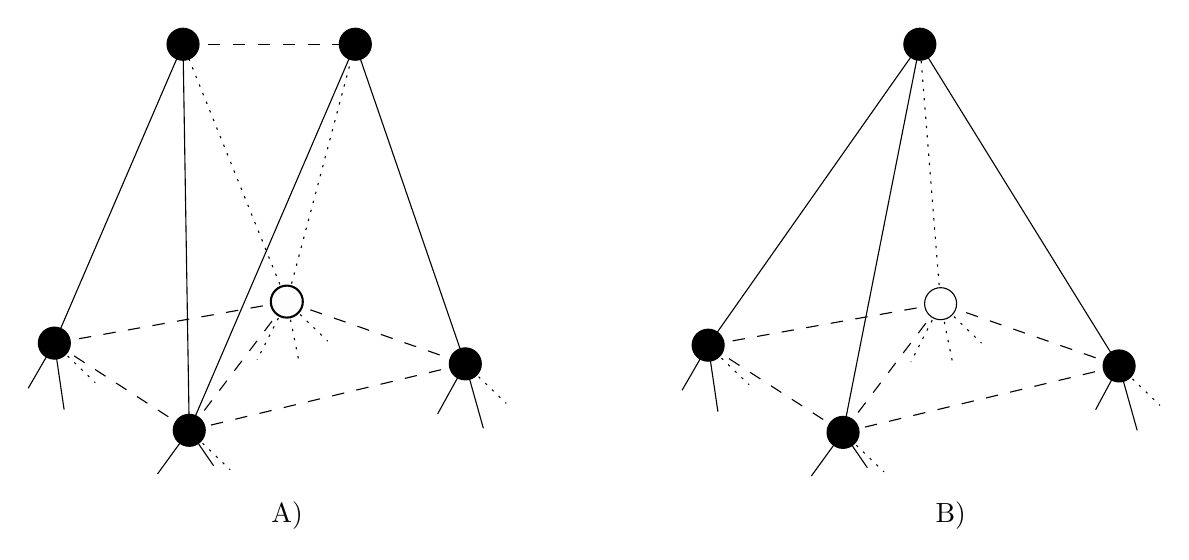
\begin{tikzpicture}[x=0.75pt,y=0.75pt,yscale=-1,xscale=1]
%uncomment if require: \path (0,300); %set diagram left start at 0, and has height of 300

%Shape: Circle [id:dp05035620766690685] 
\draw  [fill={rgb, 255:red, 0; green, 0; blue, 0 }  ,fill opacity=1 ] (62,198.71) .. controls (62,194.45) and (65.45,191) .. (69.71,191) .. controls (73.97,191) and (77.42,194.45) .. (77.42,198.71) .. controls (77.42,202.97) and (73.97,206.42) .. (69.71,206.42) .. controls (65.45,206.42) and (62,202.97) .. (62,198.71) -- cycle ;
%Shape: Circle [id:dp4686949908608724] 
\draw  [fill={rgb, 255:red, 0; green, 0; blue, 0 }  ,fill opacity=1 ] (260,208.71) .. controls (260,204.45) and (263.45,201) .. (267.71,201) .. controls (271.97,201) and (275.42,204.45) .. (275.42,208.71) .. controls (275.42,212.97) and (271.97,216.42) .. (267.71,216.42) .. controls (263.45,216.42) and (260,212.97) .. (260,208.71) -- cycle ;
%Shape: Circle [id:dp6346407819557212] 
\draw  [fill={rgb, 255:red, 0; green, 0; blue, 0 }  ,fill opacity=1 ] (127,240.71) .. controls (127,236.45) and (130.45,233) .. (134.71,233) .. controls (138.97,233) and (142.42,236.45) .. (142.42,240.71) .. controls (142.42,244.97) and (138.97,248.42) .. (134.71,248.42) .. controls (130.45,248.42) and (127,244.97) .. (127,240.71) -- cycle ;
%Shape: Circle [id:dp7195706612724979] 
\draw  [fill={rgb, 255:red, 0; green, 0; blue, 0 }  ,fill opacity=1 ] (207,54.71) .. controls (207,50.45) and (210.45,47) .. (214.71,47) .. controls (218.97,47) and (222.42,50.45) .. (222.42,54.71) .. controls (222.42,58.97) and (218.97,62.42) .. (214.71,62.42) .. controls (210.45,62.42) and (207,58.97) .. (207,54.71) -- cycle ;
%Shape: Circle [id:dp5765916913550351] 
\draw  [fill={rgb, 255:red, 0; green, 0; blue, 0 }  ,fill opacity=1 ] (124,54.71) .. controls (124,50.45) and (127.45,47) .. (131.71,47) .. controls (135.97,47) and (139.42,50.45) .. (139.42,54.71) .. controls (139.42,58.97) and (135.97,62.42) .. (131.71,62.42) .. controls (127.45,62.42) and (124,58.97) .. (124,54.71) -- cycle ;
%Straight Lines [id:da37759380231525297] 
\draw    (69.71,198.71) -- (131.71,54.71) ;
%Straight Lines [id:da9376744471268476] 
\draw    (134.71,240.71) -- (131.71,54.71) ;
%Straight Lines [id:da32775565099984716] 
\draw    (134.71,240.71) -- (214.71,54.71) ;
%Straight Lines [id:da6041709533066874] 
\draw    (267.71,208.71) -- (214.71,54.71) ;
%Straight Lines [id:da6317245362903968] 
\draw  [dash pattern={on 0.84pt off 2.51pt}]  (181.71,178.71) -- (214.71,54.71) ;
%Straight Lines [id:da8371754810800066] 
\draw  [dash pattern={on 0.84pt off 2.51pt}]  (181.71,178.71) -- (131.71,54.71) ;
%Straight Lines [id:da4677958006621281] 
\draw  [dash pattern={on 4.5pt off 4.5pt}]  (131.71,54.71) -- (214.71,54.71) ;
%Shape: Circle [id:dp4606114956520594] 
\draw  [fill={rgb, 255:red, 0; green, 0; blue, 0 }  ,fill opacity=1 ] (377,199.71) .. controls (377,195.45) and (380.45,192) .. (384.71,192) .. controls (388.97,192) and (392.42,195.45) .. (392.42,199.71) .. controls (392.42,203.97) and (388.97,207.42) .. (384.71,207.42) .. controls (380.45,207.42) and (377,203.97) .. (377,199.71) -- cycle ;
%Shape: Circle [id:dp042173618901185095] 
\draw  [fill={rgb, 255:red, 0; green, 0; blue, 0 }  ,fill opacity=1 ] (575,209.71) .. controls (575,205.45) and (578.45,202) .. (582.71,202) .. controls (586.97,202) and (590.42,205.45) .. (590.42,209.71) .. controls (590.42,213.97) and (586.97,217.42) .. (582.71,217.42) .. controls (578.45,217.42) and (575,213.97) .. (575,209.71) -- cycle ;
%Shape: Circle [id:dp8694133446914236] 
\draw  [fill={rgb, 255:red, 0; green, 0; blue, 0 }  ,fill opacity=1 ] (442,241.71) .. controls (442,237.45) and (445.45,234) .. (449.71,234) .. controls (453.97,234) and (457.42,237.45) .. (457.42,241.71) .. controls (457.42,245.97) and (453.97,249.42) .. (449.71,249.42) .. controls (445.45,249.42) and (442,245.97) .. (442,241.71) -- cycle ;
%Shape: Circle [id:dp0025939920836203223] 
\draw  [fill={rgb, 255:red, 0; green, 0; blue, 0 }  ,fill opacity=1 ] (479,54.71) .. controls (479,50.45) and (482.45,47) .. (486.71,47) .. controls (490.97,47) and (494.42,50.45) .. (494.42,54.71) .. controls (494.42,58.97) and (490.97,62.42) .. (486.71,62.42) .. controls (482.45,62.42) and (479,58.97) .. (479,54.71) -- cycle ;
%Straight Lines [id:da3954724659164921] 
\draw    (384.71,199.71) -- (486.71,54.71) ;
%Straight Lines [id:da4143192701416989] 
\draw    (449.71,241.71) -- (486.71,54.71) ;
%Straight Lines [id:da1707961218406232] 
\draw    (582.71,209.71) -- (486.71,54.71) ;
%Straight Lines [id:da9767630428206302] 
\draw  [dash pattern={on 0.84pt off 2.51pt}]  (496.71,179.71) -- (486.71,54.71) ;
%Straight Lines [id:da3253590056138286] 
\draw    (69.71,198.71) -- (57.13,220.46) ;
%Straight Lines [id:da778450447328664] 
\draw    (69.71,198.71) -- (74.42,230.75) ;
%Straight Lines [id:da8966165151524572] 
\draw    (134.71,240.71) -- (146.42,257.75) ;
%Straight Lines [id:da6099838312195625] 
\draw    (134.71,240.71) -- (119.42,261.75) ;
%Straight Lines [id:da7366949201203545] 
\draw    (267.71,208.71) -- (254.42,232.75) ;
%Straight Lines [id:da311550171749017] 
\draw    (267.71,208.71) -- (276.42,239.75) ;
%Straight Lines [id:da04066918314392831] 
\draw  [dash pattern={on 0.84pt off 2.51pt}]  (69.71,198.71) -- (89.42,217.75) ;
%Straight Lines [id:da08830304748249895] 
\draw  [dash pattern={on 0.84pt off 2.51pt}]  (134.71,240.71) -- (154.42,259.75) ;
%Straight Lines [id:da7835811470259997] 
\draw  [dash pattern={on 0.84pt off 2.51pt}]  (267.71,208.71) -- (287.42,227.75) ;
%Straight Lines [id:da02759266210026068] 
\draw  [dash pattern={on 0.84pt off 2.51pt}]  (181.71,178.71) -- (201.42,197.75) ;
%Straight Lines [id:da706959282712948] 
\draw  [dash pattern={on 0.84pt off 2.51pt}]  (181.71,178.71) -- (167.42,206.75) ;
%Straight Lines [id:da8208704819413917] 
\draw  [dash pattern={on 0.84pt off 2.51pt}]  (181.71,178.71) -- (187.42,206.75) ;
%Straight Lines [id:da07456001189898642] 
\draw    (582.71,209.71) -- (571.42,230.75) ;
%Straight Lines [id:da3316922572836051] 
\draw    (582.71,209.71) -- (591.42,240.75) ;
%Straight Lines [id:da1252397036767542] 
\draw  [dash pattern={on 0.84pt off 2.51pt}]  (582.71,209.71) -- (602.42,228.75) ;
%Straight Lines [id:da3180071623641] 
\draw  [dash pattern={on 0.84pt off 2.51pt}]  (449.71,241.71) -- (469.42,260.75) ;
%Straight Lines [id:da7250819116454129] 
\draw    (449.71,241.71) -- (461.42,258.75) ;
%Straight Lines [id:da6231164001454006] 
\draw    (449.71,241.71) -- (434.42,262.75) ;
%Straight Lines [id:da04701061115013094] 
\draw    (384.71,199.71) -- (372.13,221.46) ;
%Straight Lines [id:da006614549315218321] 
\draw    (384.71,199.71) -- (389.42,231.75) ;
%Straight Lines [id:da006487038172509729] 
\draw  [dash pattern={on 0.84pt off 2.51pt}]  (384.71,199.71) -- (404.42,218.75) ;
%Straight Lines [id:da830645107363633] 
\draw  [dash pattern={on 0.84pt off 2.51pt}]  (496.71,179.71) -- (482.42,207.75) ;
%Straight Lines [id:da6991708565197023] 
\draw  [dash pattern={on 0.84pt off 2.51pt}]  (496.71,179.71) -- (502.42,207.75) ;
%Straight Lines [id:da051658894042332815] 
\draw  [dash pattern={on 0.84pt off 2.51pt}]  (496.71,179.71) -- (516.42,198.75) ;
%Straight Lines [id:da19736423979973872] 
\draw  [dash pattern={on 4.5pt off 4.5pt}]  (69.71,198.71) -- (181.71,178.71) ;
%Straight Lines [id:da6335140704697866] 
\draw  [dash pattern={on 4.5pt off 4.5pt}]  (134.71,240.71) -- (181.71,178.71) ;
%Straight Lines [id:da7910079796960376] 
\draw  [dash pattern={on 4.5pt off 4.5pt}]  (134.71,240.71) -- (69.71,198.71) ;
%Straight Lines [id:da08773453161319089] 
\draw  [dash pattern={on 4.5pt off 4.5pt}]  (267.71,208.71) -- (134.71,240.71) ;
%Straight Lines [id:da21087372399360982] 
\draw  [dash pattern={on 4.5pt off 4.5pt}]  (181.71,178.71) -- (267.71,208.71) ;
%Straight Lines [id:da7846922422464511] 
\draw  [dash pattern={on 4.5pt off 4.5pt}]  (384.71,199.71) -- (449.71,241.71) ;
%Straight Lines [id:da9700664435813178] 
\draw  [dash pattern={on 4.5pt off 4.5pt}]  (384.71,199.71) -- (496.71,179.71) ;
%Straight Lines [id:da38856321477926614] 
\draw  [dash pattern={on 4.5pt off 4.5pt}]  (449.71,241.71) -- (496.71,179.71) ;
%Straight Lines [id:da8134429167548131] 
\draw  [dash pattern={on 4.5pt off 4.5pt}]  (582.71,209.71) -- (496.71,179.71) ;
%Straight Lines [id:da6317419675913276] 
\draw  [dash pattern={on 4.5pt off 4.5pt}]  (582.71,209.71) -- (449.71,241.71) ;
%Shape: Circle [id:dp7792019437950772] 
\draw  [fill={rgb, 255:red, 255; green, 255; blue, 255 }  ,fill opacity=1 ] (489,179.71) .. controls (489,175.45) and (492.45,172) .. (496.71,172) .. controls (500.97,172) and (504.42,175.45) .. (504.42,179.71) .. controls (504.42,183.97) and (500.97,187.42) .. (496.71,187.42) .. controls (492.45,187.42) and (489,183.97) .. (489,179.71) -- cycle ;
%Shape: Circle [id:dp08259773242466917] 
\draw  [fill={rgb, 255:red, 253; green, 253; blue, 253 }  ,fill opacity=1 ][line width=0.75]  (174,178.71) .. controls (174,174.45) and (177.45,171) .. (181.71,171) .. controls (185.97,171) and (189.42,174.45) .. (189.42,178.71) .. controls (189.42,182.97) and (185.97,186.42) .. (181.71,186.42) .. controls (177.45,186.42) and (174,182.97) .. (174,178.71) -- cycle ;

% Text Node
\draw (173,274) node [anchor=north west][inner sep=0.75pt]   [align=left] {A)};
% Text Node
\draw (493,274) node [anchor=north west][inner sep=0.75pt]   [align=left] {B)};


\end{tikzpicture}

\caption{Procedure to remove short segments. The dotted lines represent edges at the back, while the dashed lines represent the edges of the triangulation. The image A shows the initial state where two vertices from the two neighbouring simplices are generated too close together. Image B shows the final state from the merging process, where this short segment is removed.}
\label{fig:merge_points}
\end{figure}

\begin{figure}[H]
    \includegraphics[width=1\textwidth]{imgs/remove_segments.pdf}
    \centering
    \caption{Example of the result of the process of removing short segments. The initial triangulation is represented in dotted blue lines, and the green lines represent the final tessellation.
    Whereas the red lines represent the segments to eliminate, and the black points represent the midpoints of each segment.
    Also, a detail of a set of segments to eliminate is shown, where it can be seen that the convergence point corresponds to the midpoint of the set of points. }
\label{fig:merge_segments}
\end{figure}

While it is true that this process removes the short segments and reduces the number of small triangles, it is also true that still existing a disparity in the size of the triangles that would be interesting to reduce.
Different triangle areas would generate a wide range of tetrahedron heights.
Generally, the smaller the triangle, the shorter the height of the tetrahedron.
The \cref{fig:3d_apexes} shows a triangulation of a set of points with a small decreasing triangle area gradient from left to right.
It also includes a representative surface generated from the apexes found from the triangulation.
It can be seen that the slope of the surface is proportional to the gradient of the triangle area and, therefore, the different heights produced by the different triangle areas.

\begin{figure}[h!]
    \includegraphics[width=0.8\textwidth]{imgs/3d_apexes.pdf}
    \centering
    \caption{Representation of the triangulation of a set of points with a decreasing triangle area gradient from left to right. From those triangles and the apexes obtained from them, a surface is generated showing that the height of each tetrahedron is proportional to the area of the triangle.}
\label{fig:3d_apexes}
\end{figure}

To mitigate this dispersion in the heights of the tetrahedra, a routine is implemented to increase the area of the smaller triangles, thus reducing the differences in the areas of the triangles.
To do this, the routine looks for the triangles that have an area smaller than a threshold.
The area of the triangles is computed as half of the norm of the cross product of the vectors that form the triangle (\cref{eq:area}).
When this area is smaller than a defined value, the vertex closer to the origin of the Cartesian coordinate system is selected.
Then, all the points that are connected to this vertex are retrieved, and the vertex is moved to the centroid of this set of points.
In the \cref{fig:small_area}, a detail of the output of this routine is shown.
In the image, the initial triangulation is represented in dotted blue lines, and the green lines represent the final tessellation.
Also, the red points represent the triangle with a small area, and the pointed vertex in cyan is the vertex that is moved to the centroid of the set of points, which is represented by the black point.
It can be observed that the new triangles have a more uniform area.
The result of this routine in the triangulation of the set of points is shown in the \cref{fig:euler} \textcolor{blue}{B} can be observed in the \cref{fig:small_area_2}.
In the figure, the initial triangulation is shown in dotted magenta lines, and the final tessellation in green lines. 
The red points represent the new positions of the vertices that have been moved to the centroid of the set of points, while the points marked caret down represent the initial distribution of the vertices.
It can be appreciated that now the triangulation is more uniform.

\begin{equation}
    \text{Area} = \frac{1}{2} \left\| \vec{AB} \times \vec{AC} \right\|
    \label{eq:area}
\end{equation}


\begin{figure}[htbp!]
    \includegraphics[width=0.4\textwidth]{imgs/small_area.pdf}
    \centering
    \caption{Example of the result of the process of increasing the area of the small triangles. The initial triangulation is represented in dotted blue lines, and the green lines represent the final tessellation. The red points represent the triangle with a small area, and the pointed vertex in cyan is the vertex that is moved to the centroid of the set of points, which is represented by the black point.}
\label{fig:small_area}
\end{figure}

\begin{figure}[!hbtp]
    \includegraphics[width=0.9\textwidth]{imgs/small_area_2.pdf}
    \centering
    \caption{Comparison between the triangulation of a section before the area relaxation procedure and after application.}
\label{fig:small_area_2}
\end{figure}

The process of removing short segments and increasing the area of the small triangles is not exclusive and can be combined to obtain a better performance.
In the \cref{fig:optimized} is shown the input and output results of the process of removing short segments and increasing the area of the small triangles.
The initial triangulation in the example is made up of 153 vertices, while only 118 remain after the process.
That is translated into a reduction from 277 simplices to 211 and a smoother and more uniform tessellation, although some small triangles remain.


\begin{figure}[!hbtp]
    \includegraphics[width=1\textwidth]{imgs/optimized.pdf}
    \centering
    \caption{Final result of the process of removing short segments and increasing the area of the small triangles. The initial triangulation is represented in dotted magenta lines, and the final tessellation in green lines. The red points represent the new positions of the vertices that have been moved to the centroid of the set of points, while the points marked caret down represent the initial distribution of the vertices.}
\label{fig:optimized}
\end{figure}

\newpage
A brief analysis of the variation of the heights and areas from the triangles in the \cref{fig:optimized} is shown in the \cref{fig:distribution}.
The blue bars represent the distribution of the heights of the tetrahedra in the initial triangulation, while the orange bars represent the distribution of the heights of the tetrahedra after the processing.
Also, the mean values of each distribution are represented by the dashed lines, cyan for the initial distribution and red for the final distribution.
A reduction in the tetrahedra of lower height and a greater concentration of heights around the mean can be seen. 
Regarding the areas, the greater presence of large areas causes the distribution to shift to the right.


\begin{figure}[!hbtp]
    \includegraphics[width=0.8\textwidth]{imgs/distributions.pdf}
    \centering
    \caption{Distribution of the heights and areas of the tetrahedra in the initial triangulation and after the process of removing short segments and increasing the area of the small triangles. The blue bars represent the distribution of the heights of the tetrahedra in the initial triangulation, while the orange bars represent the distribution of the heights of the tetrahedra after the processing. Also, the mean values of each distribution are represented by the dashed lines, cyan for the initial distribution and red for the final distribution.}
\label{fig:distribution}
\end{figure}

In view of the results shown in the figure above, it is questionable whether this vertex processing really helps to reduce the point density, or even if it makes sense. 
As mentioned above, in the example shown, the number of vertices has been reduced from 153 to 118, which is a reduction of 22.9\%.
Additionally, the number of simplices has been reduced from 277 to 211, which is a reduction of 23.8\%.
But the question is whether this reduction is significant enough to justify the processing of the vertices.
In order to answer this question, it is necessary to look at the \cref{eq:euler_3}.
From this equation can be noticed that the number of simplices generated is almost twice the number of vertices.
Then, if the goal of this process was to keep the vertex density constant in each iteration, the number of vertices should be reduced by half.
In the example shown, the number of vertices has been reduced by almost a quarter, which is not enough to keep the vertex density constant.
It is questionable whether it is only in the example used that the desired reduction is not achieved, but perhaps in other situations it is. 
Or that in higher layers, the reduction achieved is such that it could compensate for the excess of points in lower layers. 
But the reality is that there can never be any assurance that such a reduction in points is achieved by this algorithm, since at no time is the number of points, or triangles, that is wanted to be obtained at the end of the processing being controlled. 
Therefore, the algorithm explained above could be considered an algorithm for improving the distribution of points, but it cannot be used to control the density of points. 
In order for an algorithm to be used to keep the point density constant, it must have a parameter implemented in its logic that indicates the desired target number of points. 
And, concerning the logic of the explained algorithm, this parameter could not be implemented. 
The algorithm could be modified so that, once nearby points have been eliminated, it would continue merging points until there are as many as indicated. 
But this would only lead to situations where the nodes have too many connections, as it does not avoid excessive point generation but only clustering at certain locations.


Other than this, in the previous section, it was explained that in order to obtain the position of each vertex, \cref{eq:opt_func_sum} was solved for each of the triangles. 
This problem is formulated in such a way that the solution obtained complies with the angularity constraints. 
Then, one could realise that it does not make sense to base the solution of the point density control on the movement of the generated points since the simple fact of moving these points may cause the angularity conditions are no longer be fulfilled. 
Therefore, it makes no sense to implement a solution that does not guarantee the fulfilment of the objectives of the initial approach. 
If there is a solution to this problem, it cannot involve the movement of the generated points. 
\end{document}